\documentclass[letterpaper,10pt,titlepage,draftclsnofoot,onecolumn,onesided] {IEEEtran}
\usepackage{listings}
\usepackage{underscore}
\usepackage[bookmarks=true]{hyperref}
\usepackage[utf8]{inputenc}
\usepackage[english]{babel}
%\usepackage{titling}
\usepackage{graphicx}
\usepackage{xcolor}
\usepackage[noadjust]{cite}
\usepackage{setspace}
\usepackage{float}
\nocite{*}
\graphicspath{ {img/} }
%\usepackage{abstract}

\newcommand{\namesigdate}[2][4cm]{%
  \begin{tabular}{@{}p{#1}@{}}
    #2 \\[2\normalbaselineskip] \hrule \\[0pt]
    {\small \textit{Signature}} \\[2\normalbaselineskip] \hrule \\[0pt]
    {\small \textit{Date}}
  \end{tabular}
}
\newcommand{\studentnamesigdate}[2][4cm]{%
  \begin{tabular}{@{}p{#1}@{}}
    #2 \\[2\normalbaselineskip] \hrule \\[0pt]
    {\small \textit{Signature}} \\[2\normalbaselineskip] \hrule \\[0pt]
    {\small \textit{Signature}} \\[2\normalbaselineskip] \hrule \\[0pt]
    {\small \textit{Signature}} \\[2\normalbaselineskip] \hrule \\[0pt]
    {\small \textit{Signature}} \\[2\normalbaselineskip] \hrule \\[0pt]
    {\small \textit{Date}}
  \end{tabular}
}

\hypersetup{
    bookmarks=false,    % show bookmarks bar?
    pdftitle={Progress Report},    % title
    pdfauthor={Cramer Smith, Sam Lichlyter, Eric Winkler, Zach Schneider},                     % author
    pdfsubject={Progress Report},                        % subject of the document
    pdfkeywords={IFT, Report, Postal}, % list of keywords
    colorlinks=true,       % false: boxed links; true: colored links
    linkcolor=black,       % color of internal links
    citecolor=black,       % color of links to bibliography
    filecolor=black,        % color of file links
    urlcolor=blue,        % color of external links
    linktoc=page            % only page is linked
} 

\lstdefinestyle{customperl}{
  belowcaptionskip=1\baselineskip,
  breaklines=true,
  frame=L,
  xleftmargin=\parindent,
  language=Perl,
  columns=fullflexible,
  showstringspaces=false,
  basicstyle=\footnotesize\ttfamily,
  keywordstyle=\bfseries\color{green!40!black},
  commentstyle=\itshape\color{purple!40!black},
  identifierstyle=\color{blue},
  stringstyle=\color{orange},
  numbers=left
}
\lstset{escapechar=@, style=customperl}

% Document Title:
\def\doctitle{A Tool to Visualize the Structure of a Codebase Using Information Foraging Theory Design Patterns}
\def\doctype{Final Report}
\def\team{Team Postal | Group \#38}

\markboth{Oregon State University}{\doctitle}

\begin{document}

\title{\Huge{\bfseries{\textsf{\doctitle}}}\\\textsf{\Large{\doctype}}\\\textsf{\large{\team}}}
\author{Cramer Smith, Sam Lichlyter, Eric Winkler, Zach Schneider}

\maketitle
\vfill

\setlength\parindent{0pt} \textbf{Abstract:} Developer tools are often complex pieces of software. 
Gathering and manipulating useful information for a programmer can often be a slow and costly process. 
By implementing Information Foraging Theory design patterns in the creation of these tools, the information collected may be more useful or produced faster. 
Information Foraging Theory is the theory and math behind the choices people make to maximize the value of the information they find versus the cost of getting that information.
The aim of this project is to develop a tool that will act as a proof of concept to this idea and increase developer efficiency.
Through the implementation of multiple IFT design patterns, the Postal team will create a developer tool that helps enforce and maintain code structure. 

\vfill

\pagebreak

\tableofcontents


\pagebreak

\section{Introduction}
\subsection{Client and Project Origins}
This project originated in August 2016 when one of the the team's members, Sam Lichlyter, was made aware of a research opportunity offered by Professor Christopher Scaffidi from Oregon State University. 
Prof. Scaffidi's primary research area is in Information Foraging Theory (IFT) which revolves around studying how humans find and utilize information sources. 
Sam, already a student researcher under Prof. Scaffidi, asked if he could create a Senior Capstone project out of IFT in a new study concerning software developers.
Prof. Scaffidi prompted Sam to identify a team and to come up with a project proposal that would develop a software tool according to the principles of IFT. 
Sam included Eric Winkler, Zach Schneider and Cramer Smith in the potential Capstone team. 
There were two proposals submitted for consideration: an interface to allow developers to read and search program log files more easily, and an extension for an IDE that would automatically organize a developers code into appropriate concerns i.e., the data layer, interface layer, and application layer.
The latter of the proposals was selected and this Capstone team was formed to undertake it.

\subsection{Project Purpose and Expectations}
A more detailed explanation of what the team was tasked with is as follows.
First, design a tool according to IFT design patterns that will help developers find and utilize information, in this case, within an IDE.
Second, build and code said tool until it is in a state where it is useful in its main purposes.
Next, organize a series of formal user tests to determine if the tool aides developers in performing a set of real world tasks.
Finally, analyze the results of the tests and, if the results are positive, write a formal research paper describing the entire process and its relationship to IFT.
Prof. Scaffidi supervised the design process in the Fall. The team met with him about once and month to check in and discuss any design questions or changes. 
Emails were exchanged a bit more often. 
He left the coding and implementation phase largely up to the team during the end of Fall through the Winter and contact was infrequent. 
Spring term saw contact pick up again as the team finalized the product with him and began arranging the necessary materials for user testing. 
Prof. Scaffidi has and will continue to directly facilitate the actual testing and analysis process until it is complete.

\subsection{Project Roles}
Throughout the year, each team member assumed and carried out various roles depending on the stage of the project. 
Every member generally contributed to all aspects of the project, but the responsibility for some areas was assumed primarily by one individual.

Sam undertook served as the team's primary client contact since the relationship had existed prior to the beginning of this project. 
He had a major role in the design and implementation of the parser component of this tool, along with Eric. 
Additionally, Sam wrote many of the grammars and rules that the parser would use to find specific data within developers' codebases. 

Zach took primary responsibility for project documentation, deadlines and general administrative work. He contributed to early iterations of the data structure used to store parsed data within the tool. 
He then transitioned to adding features to the user interface (UI) and testing various use cases within it.

Cramer did much of the research into which IDE the tool would be developed for. 
Once Visual Studio Code was decided upon by the team as the platform for this project, he also created the core of code required to launch and include extensions within that platform. 
Cramer deployed each iteration of the tool to the Microsoft VS Code Extension Gallery online when various project milestones were reached.

Eric served as overall project architect, coming up with the general structure of the project from the original proposal and changing it as necessary throughout the year. 
He worked with Sam in building the parser and created the core of the UI and Electron window code. 
When the parser was modified in the middle of the year, he also re-worked the data structure system being used.


\section{Original Requirements and Timeline}

\section{Updates to Requirements and Timeline}
\begin{center}
	\begin{singlespace}
		\begin{tabular}{ |  p{0.25\linewidth}  |  p{0.25\linewidth}  | p{0.25\linewidth} | p{0.25\linewidth} |}
		\hline
		Topic & title & title & title \\ \hline
		
			ROW TITLE
		& 
			\begin{itemize}
				\item 
			\end{itemize}
		& 
			\begin{itemize}
				\item 
			\end{itemize}
		&
			\begin{itemize}
				\item 
			\end{itemize} 
		\\ \hline
			Next Row Title
		& 
			\begin{itemize}
				\item 
			\end{itemize}
			%etc...
			
			\\ \hline
		\end{tabular}
	\end{singlespace}
\end{center}

\section{Design Documents and Changes}

\section{Technology Review and Changes}

\section{Weekly Blog Posts}
	\input{blogposts}	
		
	

\section{Engineering Expo Poster}
%leave this blank, we'll just print this out separately in color

\section{Project Documentation}

\section{Resources and Technologies}

\section{Learning and Overall Experience}
\subsection{Sam Lichlyter}

\subsection{Zach Schneider}

\subsection{Cramer Smith}

\subsection{Eric Winkler}

\pagebreak
\section{Appendix 1}
\section{Code Samples}
	\subsection{Example Grammar}
	This is the default grammar that parses HTML and PHP files for divs and links.
	
	\begin{lstlisting}
{
    "id" : 0,
    "title" : "html",
    "filetypes" : ["html", "php"],
    "rules" : [{
            "title": "div",
            "type": "tagged",
            "options" : {
                "tagStart": "<div",
                "namedOption" : "id=\"(.+?)\"",
                "tagEnd": ">",
                "closingTag": "</div>",
                "nodeColor": "blue"
            }
        }, {
            "title": "href link",
            "type" : "link",
            "options" : {
                "link": "href=[\"](.+?)[\"]",
                "nodeColor": "blue"
            }
        }, {
            "title": "includes link",
            "type": "link",
            "options": {
                "link": "include=[\"](.+?)[\"]",
                "nodeColor": "blue"
            }
        }, {
            "title": "body",
            "type": "tagged",
            "options" : {
                "tagStart": "<body",
                "tagEnd": ">",
                "closingTag": "</body>",
                "nodeColor": "blue"
            }
        }
    ]
}
	\end{lstlisting}

	\pagebreak
	\subsection{Recursive Get All Links}
	This function grabs all the links from the data structure of a specified file struct and it's children.
	\begin{lstlisting}
// Recursive function to get all links from this and children
function getAllLinksFromFileStructRecursive(FileStructID) {
    var links = [];

    // check parent
    if (DFS[FileStructID].links.length > 0) {
        for (var i = 0; i < DFS[FileStructID].links.length; i++) {
            var link = DFS[FileStructID].links[i];
            links.push(link);
        }
    }

    // check children
    if (DFS[FileStructID].subContainers.length > 0) {
        var childLinks = [];
        for (var i = 0; i < DFS[FileStructID].subContainers.length; i++) {
            var childFileStructID = DFS[DFS[FileStructID].subContainers[i].toFileStructid].id;
            childLinks = getAllLinksFromFileStructRecursive(childFileStructID);

            // push what we found to parents link list
            for (var j = 0; j < childLinks.length; j++) {
                links.push(childLinks[j]);
            }

        }
    } 

    return links;
}
	\end{lstlisting}

\pagebreak
\section{Appendix 2}	
\section{Images}
	\begin{figure}[H]
		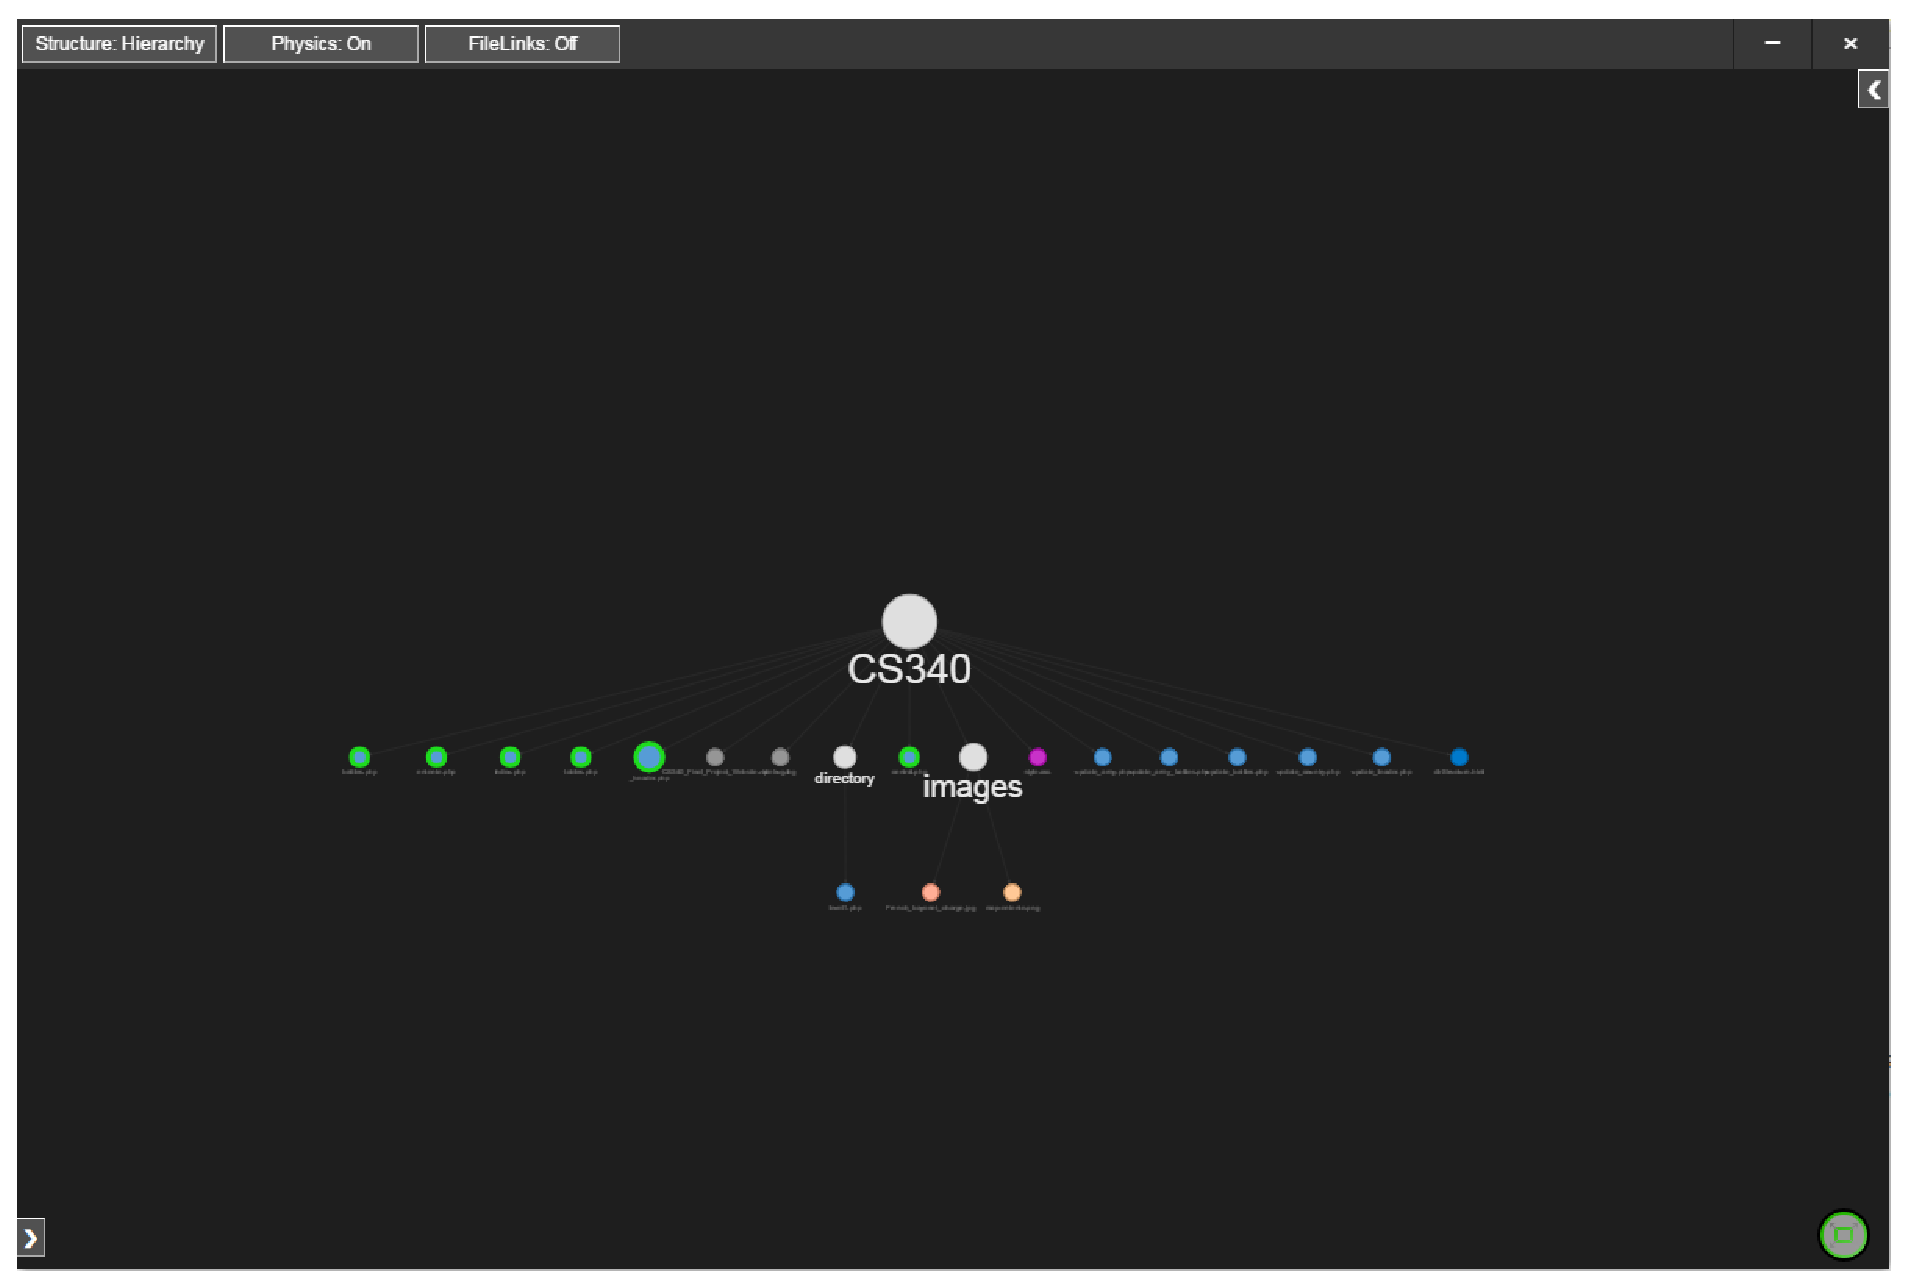
\includegraphics[width=400px]{PostalUI}
		\caption{Visualization Interface}  
	\end{figure}
	
	\begin{figure}[H]
		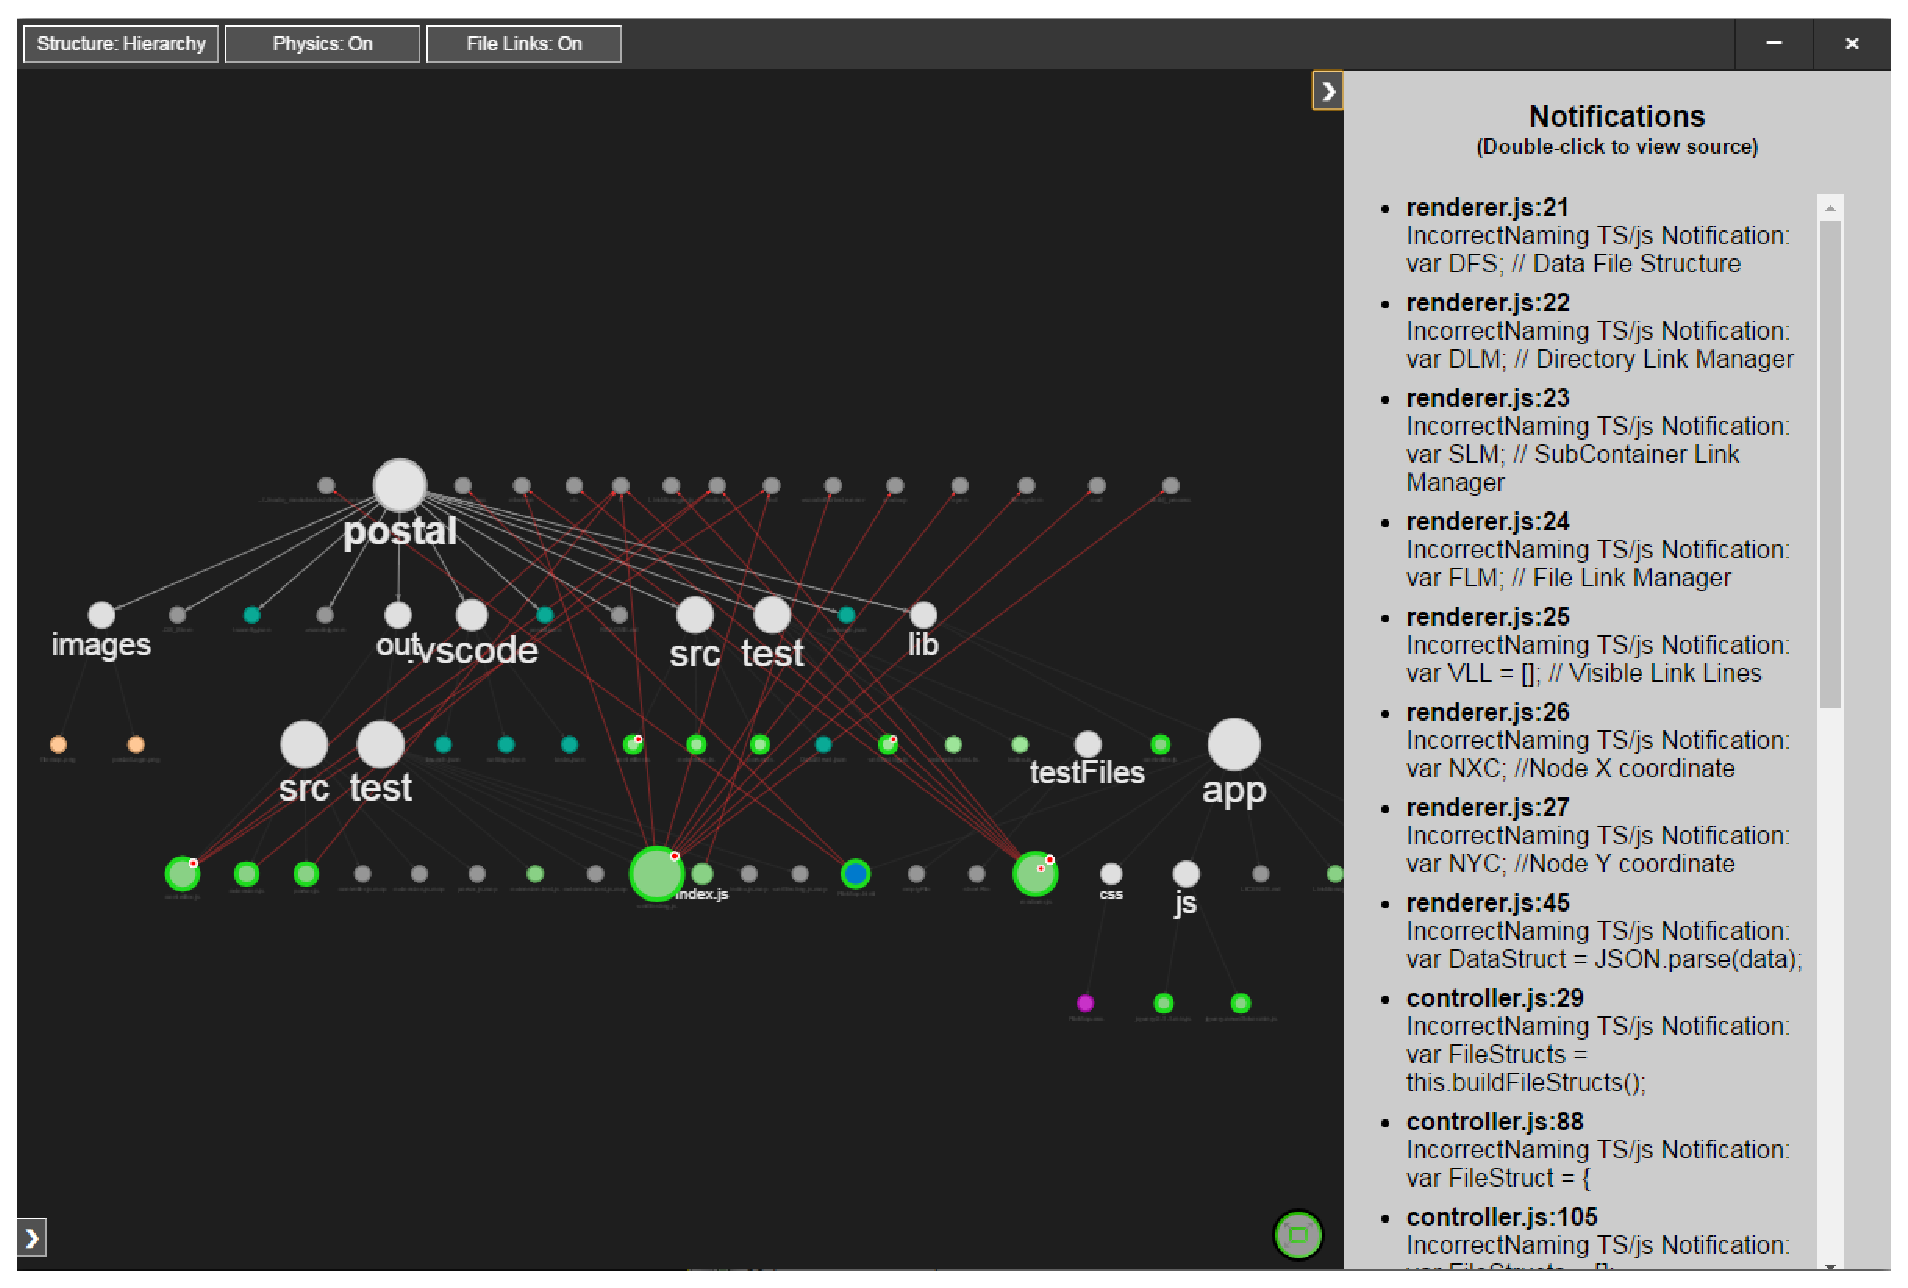
\includegraphics[width=400px]{PostalNotification}
		\caption{Notification Interface}  
	\end{figure}
	
	\begin{figure}[H]
		\includegraphics[width=400px]{UpdatedDataStruct}
		\caption{Updated Data Structure}
	\end{figure}
	
\pagebreak
\bibliographystyle{IEEEtran}
\bibliography{progress-report-team38}


\end{document}

